\documentclass[letterpaper]{article}
\usepackage{adjustbox}
 % DO NOT CHANGE THIS
\usepackage{aaai20}  % DO NOT CHANGE THIS
\usepackage{times}  % DO NOT CHANGE THIS
\usepackage{helvet} % DO NOT CHANGE THIS
\usepackage{courier}  % DO NOT CHANGE THIS
\usepackage[hyphens]{url}  % DO NOT CHANGE THIS
\usepackage{graphicx} % DO NOT CHANGE THIS
\urlstyle{rm} % DO NOT CHANGE THIS
\def\UrlFont{\rm}  % DO NOT CHANGE THIS
\usepackage{graphicx}  % DO NOT CHANGE THIS
\frenchspacing  % DO NOT CHANGE THIS
\setlength{\pdfpagewidth}{8.5in}  % DO NOT CHANGE THIS
\setlength{\pdfpageheight}{11in}  % DO NOT CHANGE THIS

\usepackage[utf8]{inputenc}
\usepackage{bbold}
\usepackage{amssymb}
\usepackage{amsmath}
\usepackage{balance}
\usepackage{tikz}
\usepackage{subfig}
\usepackage{bbm}
\usepackage{enumitem}
\usepackage{appendix}

\DeclareMathOperator*{\argmax}{arg\,max}
\providecommand{\TODO}[1]{\textcolor{red}{\textbf{#1}}}




\title{A Probabilistic Simulator of Spatial Demand for Product Allocation}

\author{Porter Jenkins \textsuperscript{\rm 1}, Hua Wei \textsuperscript{\rm 1}, J. Stockton Jenkins \textsuperscript{\rm 2}, Zhenhui Li \textsuperscript{\rm 1} \\
\textsuperscript{\rm 1} Penn State University \\
\textsuperscript{\rm 2} Brigham Young University \\%If you have multiple authors and multiple affiliations
}


\begin{document}
\maketitle

\begin{abstract}
Connecting consumers with relevant products is a very important problem in both online and offline commerce. In physical retail, product placement is an effective way to connect consumers with products. However, selecting product locations within a store can be a tedious process. Moreover, learning important spatial patterns in offline retail is challenging due to the scarcity of data and the high cost of exploration and experimentation in the physical world. To address these challenges, we propose a stochastic model of spatial demand in physical retail. We show that the proposed model is more predictive of demand than existing baselines. We also perform a preliminary study into different automation techniques and show that an optimal product allocation policy can be learned through Deep Q-Learning.

\end{abstract}



\section{Introduction}
From cleaning robots to self-driving cars, autonomous and semi-autonomous agents are becoming increasingly prevalent~\cite{stone2016artificial}. People's understanding of such agents' behaviors can increase their trust in the agents and their ability to collaborate with them~\cite{devin2016implemented,glass2008toward}. An understanding of an agent's behavior could also support people in tasks such as choosing between alternative agents and determining when the agent can be trusted with performing a task autonomously and when the user's attention is needed. For example, if a user can anticipate the behavior of  a self-driving car in different scenarios, she could be more prepared to take control in situations where the car might not perform well on its own.

While prior work has suggested ways to explain individual decisions of an agent to a person~\cite{khan2009minimal,khan2011automatically}, these approaches do not convey a ``global'' view of an agent's policy. Similarly, recent methods for interpretable machine learning~\cite{vellido2012making,doshi2017towards} typically explain a single decision made by a model, e.g. by presenting a simplified model which justifies decisions in a certain region in the space~\cite{ribeiro2016model}. In this paper, we introduce the problem of providing users with a summary of an agent's behavior. This approach aims to provide users with an overview of the agent's global strategy rather than explaining specific decisions  after the fact. 

A trivial way of communicating an agent's behavior is to show past executions or simulations. This approach, however, has important drawbacks. First, many of the situations an agent encounters might be uninteresting to a person (e.g., a self-driving car stuck in traffic for an hour). Second, reviewing long execution traces will require a person to spend a significant amount of time, and people might give up early, or not pay attention, potentially missing important states. Therefore, we seek solutions that extract \emph{effective} summaries which show the actions taken by the agent in key scenarios. Such summaries can reduce the human effort required to review the agent's behavior, while still providing sufficient information about its capabilities. We note that this is analogous to the approach taken in many settings in which people need to assess the performance of other people. For example, sports scouting agencies typically prepare videos that include highlights from players' games to demonstrate their skills\footnote{e.g.,  \url{https://www.youtube.com/watch?v=gX3e0UM-OeM}. We note that while such scouting videos are often biased to showcase only successful actions, we intend that summaries of agent behavior will include states that demonstrates their behavior in different states of interest, whether successful or not.}.  

%The approach of generating summaries that highlight the capabilities of agents is analogous to other settings in which people need to review the performance of other people. For example, sports scouting agencies prepare videos that include highlights from players' games to demonstrate their skills.\footnote{e.g.,  \url{https://www.youtube.com/watch?v=gX3e0UM-OeM}.}

We developed ``HIGHLIGHTS'', an algorithm that extracts important states from an execution trace of an agent in an online manner. Intuitively, a state is important if different actions in that states can lead to substantially different outcomes for the agent. For example, deciding which turn to take when driving in a city will not be considered important if taking the next turn will result in a similar arrival time; deciding whether to exit a highway will be considered more important, as missing the exit can result in a significant delay. Our approach assumes that HIGHLIGHTS has access to the agent's strategy which is described using a  Markov Decision Process (MDP) policy, and quantifies the importance of states based on the agent's Q-values. To provide more context to the user, rather than showing important states in isolation, the algorithm extracts a trajectory that includes neighboring states and composes a summary of the agent's behavior from these trajectories.

We used HIGHLIGHTS to create summaries of agents playing Mrs. Pacman~\cite{rohlfshagen2011ms} and evaluated these summaries in a human-subject experiment. We compared HIGHLIGHTS summaries with two baselines. One baseline generated summaries by extracting random trajectories of the agent, which will, on average, include states that are more likely to be encountered. The other baseline generated summaries by extracting the first trajectories the agent encountered, which is akin to having a user watch the agent until she runs out of time. In the experiment, participants were shown summaries of different Pacman agents which varied in their performance, and were asked to select an agent to play on their behalf.  They were also asked to rate the helpfulness of different summaries for evaluating an agent's capabilities. 
%They were also shown pairs of summaries of the \emph{same} Pacman agent and were asked to subjectively assess how helpful each of the summaries is for understanding that agent's capabilities. 
Our results show that HIGHLIGHTS led to improved objective performance of participants: they were significantly more likely to choose the better performing agent when the HIGHLIGHTS summaries were shown. HIGHLIGHTS summaries were also rated as more helpful by the study participants. 

%can be condensed to two sentences if needed
One limitation of the HIGHLIGHTS algorithm is that it does not consider the diversity of states in the summary, and therefore if important states are similar to each other, the summary will consist of similar trajectories, thus conveying less new information to users. To mitigate this problem, we developed a variant of the HIGHLIGHTS algorithm which, in addition to state importance, takes into consideration the similarity of the state to other states in the summary. This extension further improved participants' ability to assess the performance of different agents.

The contributions of the paper are threefold: (1) we introduce and formalize the problem of summarizing an agent's behavior to people; (2) we develop HIGHLIGHTS and HIGHLIGHTS-DIV, algorithms that automatically extract summaries of an agent's policy, and (3) we conduct human-subject experiments, showing that summaries generated by HIGHLIGHTS and HIGHLIGHTS-DIV were preferred by participants and improved their ability to assess the capabilities of agents compared to the baseline summaries.

\section{Problem Definition}\label{prob-def}
In the following section, we provide a formal definition of the optimal allocation problem. Additionally, we define the necessary components of our reinforcement learning agent: the state space, action space, reward function, and state transition function.
\subsection{Optimal Allocation Problem}

In a physical retail environment $\mathcal{R}$ with a set of $n$ spatial regions, we represent the environment with a spatial graph $\mathcal{R} = (\mathcal{V}, \mathcal{E})$, where each region $r_i\in \mathcal{V}$ is a vertex in the graph, the spatial neighboring relation between two regions $r_i$ and $r_j$ are represented as $e_{ij}\in \mathcal{V}$. From $\mathcal{G}$, we can construct the adjacency matrix, $\textbf{A}$.

Additionally, we observe a set of $k$ products, $\mathcal{M} = \{m_j : 0 < j <=k\}$ that are sold. For each product, $m_j$, we know the retail price, $p_j$. 

The decision process faced by the retailer is to allocate each product in $\mathcal{M}$ across regions in $\mathcal{R}$. We define the allocation policy as a function $f$:

\begin{equation}
    f: \mathcal{R} \times \mathcal{M} \rightarrow \mathcal{Z}
\end{equation}
\begin{equation}
    \mathcal{Z} = \{\langle r_i, p_j \rangle , ... \langle r_w, p_q \rangle \}
\end{equation}

Where $\mathcal{Z}$ is the set of selected product region, such that $w <= n$, $q <= k$ and $\mathcal{Z} \subseteq \mathcal{R} \times \mathcal{M}$. This function is typically dynamic over time, which we denote as $f^{t}$. To simplify computation, we treat $\mathcal{Z}^{t}$ as an $(n \times k)$ grid and refer to it as the board configuration at time, $t$. An optimal retail strategy is to find the allocation policy that maximizes revenue:

\begin{equation}
    f^{\ast} = \sum_{t}^{T} \argmax_{f^{t}} \sum_{i, j \in f^{t}(\mathcal{R}, \mathcal{M})} p_j q_i
\end{equation}

where $p_j$ is the price for product $m_j$, and $q_i$ is the quantity sold in region $r_i$ and $T$ is the future time horizon of analysis. The main idea of the current work is to discover the long-term, optimal allocation policy, $f^{\ast}$ from data.

\subsection{Optimal Allocation as a Markov Decision Process}
We believe that the optimal allocation problem is well suited for reinforcement learning because the RL agent is designed for sequential decision making that maximizes expected discounted reward over time. We frame the inputs as a Markov Decision Process (MDP). An MDP is defined by the tuple $\langle \mathcal{S}, \mathcal{A}, P, r, \delta  \rangle$, where $\mathcal{S}$ is the state space, $\mathcal{A}$ is the set of possible actions, $P$ is the (typically unkown) state transition function, $r$ is the reward function and $\delta \in [0,1]$ is the discount factor. 

\begin{itemize}
    \item \textbf{State} At each time, $t$, we observe the state of the retail environment, $\mathcal{E}$. We define the state, $s_t \in \mathcal{S}$, as the tuple of state features, $s_t = \langle \mathcal{Z}^{{t}}, d^{t}, \textbf{g}^{(t-1)}  \rangle$, where $\mathcal{Z}^{{t}}$ is the current board configuration, $d^t$ is the current day of the week (e.g., Sunday $\rightarrow$ 0), and $\textbf{g}^{(t-1)}$ is a vector denoting the revenue at the previous time, $(p_j q_i)^{(t-1)} \forall z \in \mathcal{Z}^t$

    \item \textbf{Action} We define the action space  $\mathcal{A} = \mathcal{R} \times \mathcal{M} \times \{-1, 1\} \cup \{0\}$, indicating ``to place'', ``take way'' or ``do nothing'' for each product, $m_j$ in each region, $r_i$.
    \item \textbf{Reward} The reward function in this case is the total product revenue at time $t$, constrained by the monetary cost, $c$, of placing a set of products in each region:
    \begin{equation}
        r(t) = \sum_{i=1}^n \sum_{j=1}^k p_j q_{ij}^{t} - c \sum_{i=1}^n \mathbbm{1}_{\mathcal{Z}}(r_i)
    \end{equation}
    
    \item \textbf{State transition function}: The state transition, $P$ is defined as $p(s^{t+1} | s^t, a^t): \mathcal{S} \times \mathcal{A} \times \mathcal{S} \rightarrow [0,1]$, which gives the probability of moving to state, $s^{(t+1)}$ given the current state and action. In the optimal allocation problem the exact transition function, $P$ is unknown since the current state, $s^t$ depends on the results of the previous time, $\textbf{g}^{(t-1)}$. We model this transition as a stochastic process.
\end{itemize}
\section{Commonsense for Zero-Shot NLVL}
\label{sec:proposedSection}

\subsection{Problem Formulation}
We denote an input video as $V$, and its grounding annotations as \(\left( Q,V_{\text{span}}\right) \), where $Q$ is the query representation and \(V_{\text{span}}\!=\!\left( t_{s},t_{e}\right)\) is the corresponding video moment span annotation, with \(t_{s}\) and \(t_{e}\) representing the start and end timestamps, respectively. Learning to localize a video moment conditioned on a query entails maximizing the expected log-likelihood of the model parameterized by \(\theta\). In its typical setting, this can be formulated as follows:
\begin{equation}
\label{eq:groundingOriginal}
    \theta ^{\ast }=\arg \max _{\theta } \mathbb{E}\left[ \log p_{\theta }\left(  V_{\text{span}} | V,Q\right) \right]. 
\end{equation}
In the zero-shot setting, the goal is to learn this task without parallel video-query annotations. Hence, the query and video moment annotations are derived from $V$, using a dynamic video moment proposal method followed by a pseudo-query generation mechanism. Formally,  \(V_{\text{span}}\,\!{=}\!\,f_{\text{span}}(V)\) and \(Q\,\!{=}\!\,f_{pq}(V_{\text{span}})\), where $f_{\text{span}}$ and $f_{\text{pq}}$ are video moment proposal and pseudo-query generation mechanisms, respectively. Given that $f_{\text{span}}$ and $f_{\text{pq}}$ are responsible for generating the annotations, the performance of the localization model heavily depends on the quality of these modules. Existing methods face challenges in aligning \(Q\) to \(V_{\text{span}}\) due to noise introduced by ungrounded pseudo-query generation mechanisms. 
To address this, we simplify \(f_{\text{pq}}\) while augmenting cross-modal understanding by leveraging external information in the form of a commonsense graph \(G_{C}(C, E)\) with \(n_c\) nodes, where \(C\!=\!\left\{c_{1}, c_{2}, \dots, c_{n_{C}}\right\}\) are the concept node vector representations and \(E\) is the set of weighted directed edges, respectively. Accordingly, learning can be formulated as
\begin{equation}
\label{eq:groundingOurs}
    \theta ^{\ast }=\arg \max _{\theta } \mathbb{E}\left[ \log p_{\theta }\left(  V_{\text{span}}| V,Q,G_{C}\right) \right].
\end{equation}

\noindent Figure \ref{fig:approach} shows both training and inference flows.
\subsection{Pseudo-supervised Setup}
\modelname first processes a raw video with a video moment proposal $f_{\text{span}}$ module that extracts important video segments capturing key events, and a pseudo-query generation $f_{\text{pq}}$ that generates text query annotations corresponding to the extracted video segments.

\paragraph{Dynamic Video Moment Proposal ($f_{\text{span}}$).}
We adopt the dynamic video moment proposal approach proposed by \citet{nam_zero-shot_2021}. Specifically, $f_{\text{span}}$ primarily comprises a k-means clustering mechanism that groups semantically similar and temporally proximal video frame features together to extract atomic moments. To obtain frame features, we consider the columns of a frame-wise similarity matrix derived from the CNN features of individual frames. We enforce temporal proximity by concatenating the frame index to the features. Composite video moments are then formed by combining neighboring atomic moments, and a subset of all possible combinations is sampled uniformly at random. The resulting set of video moments corresponds to $V_{\text{span}}$.

\paragraph{Pseudo-query Generation ($f_{\text{pq}}$).} The pseudo-query is constructed as a collection of objects present in the video. To generate the pseudo-query, we employ an off-the-shelf object detector, enabling the extraction of pertinent objects in \(V_{\text{span}}\). We adopt a top-$k$ strategy to sample the $k$ most probable object predictions associated with the query \query.

\paragraph{Video Encoder.}
We uniformly sample $T$ frames from $V$ and extract their CNN (\eg, I3D~\cite{qian_locate_2022}) features. These features are contextually encoded using a video encoder ${\phi}_{v}$ to yield frame features ${\phi}_{v}(V)\!=\!\left\{ v_{1},v_{2},\ldots,v_{T}\right\}$ where $v_{i}\in\mathbb{R}^{d}$, and $d$ is the common video/query encoding dimension. We implement ${\phi}_{v}$ as a GRU-based encoder.

\paragraph{Query Encoder.}
Our pseudo-query $Q$, composed of up to $k$ tokens, is encoded using a query encoder ${\phi}_{q}$ that generates query embeddings ${\phi}_{q}(Q)\!=\!\left\{ q_{1},q_{2},\ldots,q_{k}\right\}$, for the top-$k$ detected objects extracted from the pseudo-query generation. Here, $q_{i}\in \mathbb{R}^{d}$ and $d$ is the common video/query encoding dimension. We implement ${\phi}_{q}$ as a bi-directional GRU-based encoder preceded by a trainable embedding layer. 

\subsection{Commonsense Enhancement Module}
\label{sec:cem}
To enrich the encoded video and query features with information grounded in commonsensical knowledge, we introduce a Commonsense Enhancement Module (CEM), pictorially described in Figure~\ref{fig:cem}. This enhancement helps inject necessary information into video and query representations, which can not just help bridge the gap between the available visual and textual cues but also provide rich information to the downstream span localization module. 

\begin{figure}[t!]
    \centering
    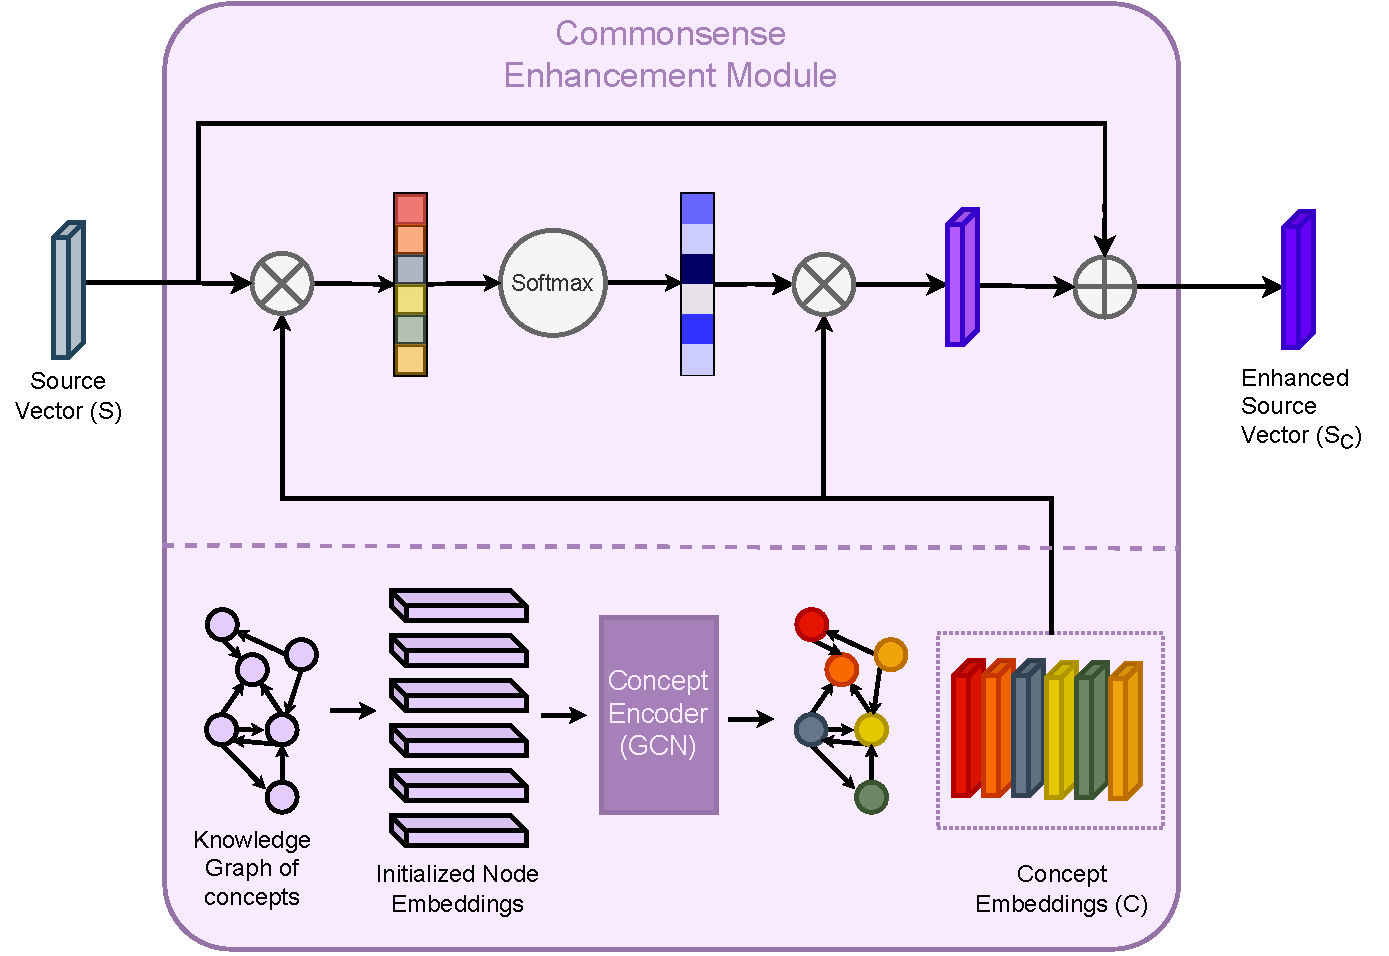
\includegraphics[width=0.8\linewidth]{figures/figure_files/Cem.pdf}
    \caption{\modelname Commonsense Enhancement Module (CEM). CEM comprises a concept encoder and an enhancement mechanism that uses the previously encoded concept vectors to update a given input vector (video/query vectors). The concept encoder employs a Graph Convolution Network for encoding the nodes (concepts) of \(G_C\). 
    }
  \label{fig:cem}
\end{figure}

CEM includes a set \(C\!=\!\left\{c_{1}, c_{2}, \dots, c_{n_{C}}\right\}\) of \(n_{C}\) concept vectors, where \(c_{i} \in \mathbb{R}^{d}\) and \(d\) is the concept feature dimension (same dimension as $\forall v_i \in V$ and $\forall q_i \in Q$). In general, given source feature vectors $S\!=\!\left\{ s_{1},s_{2},\ldots,s_{n}\right\}$ with individual feature vectors $s_{i \in [1,n]} \in \mathbb{R}^{d}$, the enhanced feature vectors $S_{C}$ are obtained using a commonsense enhancement mechanism $\phi_{C}$.
We implement this commonsense enhancement step $\phi_{C}$ as a cross-attention mechanism that enriches source input features, attending over $S$ guided by the commonsense concept vectors $C$, \ie, 
\begin{equation}
\label{eq:cenhance}
\scalemath{1}{
    }
    S_{C} = S + \phi_{C}(S) = S + \sigma \left( \frac{SW_{Q}(CW_{K})^{T}}{\sqrt{d}} \right) C W_{V},
\end{equation}
where $\sigma$ is a softmax activation, \(W_{Q}\), \(W_{K}\), \(W_{V}\) are trainable matrices and \(d\) is the common dimension of the vectors \(S\) and \(C\). In our setting, the source feature vectors $S$ are either video $V$ or pseudo-query $Q$ features. We build separate enhancement mechanisms for $V$ and $Q$, \ie, the projection matrices \(W_{Q}\), \(W_{K}\), \(W_{V}\) are not shared between $Q$ and $V$. We elaborate more on the rationale in the appendix.
The enriched video and pseudo-query features are denoted as \(V_{C}\!=\!\phi_{C_{\text{vid}}}(V)\) and \(Q_{C}\!=\!\phi_{C_{\text{pq}}}(Q)\), respectively.

\paragraph{Concept Encoder.}
The concept vectors \(C\) mentioned above are feature representations that internally form the nodes of the commonsense graph, \(G_C\). Accordingly, graph \(G_{C}\) is represented as a matrix, where \(G_{C(i,j)}\) represents the total number of directed relational edges between \(c_{i},c{j} \in C\) that start at \(c_i\) and end at \(c_j\). To encode the commonsense information, we employ Graph Convolutional Networks (GCN) \cite{hammond_wavelets_2011}. The concept encoder is composed of $L$ graph convolution layers, each of which performs a convolution step
\begin{equation}
\scalemath{1}{
    C^{\left(l+1\right)}=\sigma \left( AC^{\left(l\right) }W^{\left( l\right) }\right),
    }
\end{equation}
where $C^{\left(l\right)}$ are node (concept) features and $W^{\left( l\right)}$ trainable weight matrix of layer $l \in [1, L]$, $\sigma$ is a nonlinear activation function, and $A$ is the adjacency matrix obtained by normalizing graph $G_C$ with the degree matrix $D$. Since $G_C$ is a directed graph, normalization can be formulated as $A\!=\!D^{-1}G_{C}$.

\paragraph{Commonsense Information.}
We use ConceptNet \cite{speer_conceptnet_2017}, a popular knowledge graph that provides information spanning various types of relationships such as physical, spatial, behavioral, \etc To ensure that the ConceptNet information utilized is relevant to themes found in the video data, we consider the set of objects available in pseudo-queries and include the top-$k$ most frequently occurring objects to be the seed concept set \(C\). We extract the  ConceptNet subgraph that includes all edges incident between the concepts in \(C\). 
We filter the edge types based on a pre-determined relation set \(R\), which is compiled to involve relations that are relevant to the nature of the video localization task, \eg, spatial (\textit{AtLocation}, \etc) and temporal (\textit{HasSubevent}, \etc) relations are useful for video understanding, while \textit{RelatedTo} and \textit{Synonym} are fairly generic relations that add little information to the localization task. Table \ref{tab:relations} shows the relations included in \(G_C\).

\paragraph{Cross-Modal Interaction Module.} The commonsense enriched video and query features, \(V_{C}\) and \(Q_{C}\), are fused with a multi-modal cross-attention mechanism. We employ a two-step fusion process. First, Query-guided Video Attention (QVA) is applied to attend over video $V_C$, and Video-guided Query Attention (VQA) attends over query $Q_C$ guided by video $V_C$, resulting in updated features $V_C'$ and $Q_C'$, respectively. Both QVA and VQA utilize Attention Dynamic Filters~\cite{rodriguez_proposal-free_2020} that adaptively modify video features, dynamically adjusting them in response to the query, and vice versa. Next, the attended features are fused using a cross-attention mechanism over $V_C'$ guided by $Q_C'$, resulting in localized video features $V_{C_{\text{loc}}}$.

\paragraph{Temporal Regression Module.}
The final step involves a regression layer that approximates $\hat{V}_{\text{span}}$. We employ attention-guided temporal regression to estimate the span of the target video moment. To find important temporal segments relevant to the query, the fused features $V_{C_{\text{loc}}}$ are temporally attended based on the query features to obtain $V_{\text{ta}}$. Then, the span boundaries are localized using a regressor implemented as a Multi-Layer Perceptron (MLP).

\begin{align}
{o}_i = \sigma\left({W}_{1} V_{C_{\text{loc}_i}} + {b}_{{1}}\right) \\
V_{\text{ta}} = \sum_{i=1}^{T} o_i V_{C_{\text{loc}_{i}}} \\
[\hat{t}_s, \hat{t}_e] = {W}_2 {V}_{\text{ta}} + {b}_{2}.
\end{align}
Here, ${W}_{1}$ and ${b}_1$ are the weight matrix and bias vector of the temporal attention MLP, $\sigma$ represents the sigmoid activation function, $V_{C_{\text{loc}_i}}$ stands for the encoded localized video features, ${V}_{\text{ta}}$ represents the temporally attended video features, ${W}_2$ and ${b}_2$ denote the weight matrix and bias vector of the regression MLP, and $[\hat{t}_s, \hat{t}_e]$ correspond to the start and end timestamps of the predicted video span $\hat{V}_{\text{span}}$.

\begin{table}[t!]
\centering
\resizebox{\linewidth}{!}{
\begin{tabular}{ll}
\toprule
\textbf{Category} & \textbf{Relations}                                                                                         \\ \toprule
Spatial           & AtLocation, LocatedNear                                                                                    \\ \midrule
Temporal          & \begin{tabular}[c]{@{}l@{}}HasSubevent, HasFirstSubevent, HasLastSubevent, HasPrerequisite\end{tabular} \\ \midrule
Functional        & UsedFor                                                                                                    \\ \midrule
Causal            & Causes                                                                                                     \\ \midrule
Motivation        & MotivatedByGoal,  ObstructedBy                                                                             \\ \midrule
Other             & CreatedBy, MadeOf                                                                                          \\ \midrule
Physical          & \begin{tabular}[c]{@{}l@{}}HasA, HasProperty, Antonym, SimilarTo\end{tabular}                      
\\ \bottomrule
\end{tabular}
}

\caption{Relations in the Commonsense Enhancement Module (CEM) grouped by categories.}
\label{tab:relations}

\end{table}
\subsection{Training and Inference}
The training objective is 
$\mathcal{L}_{loc} = \mathcal{L}_{treg}+\lambda \mathcal{L}_{ta},$ where \(\lambda\) is a balancing hyperparameter, \(\mathcal{L}_{ta}\) is a temporal attention guided loss and \(\mathcal{L}_{treg}\) is the regression loss.  The temporal attention-guided loss is defined as
\begin{equation}
\label{tatt}
\mathcal{L}_{ta} = \frac{\sum^{T}_{i=1}g_{i}\log \left( a_{i}\right)}{\sum^{T}_{i=1}g_{i}},
\end{equation}
where \(a_{i}\) is the attention weight for video frame \(v_{i}\) and \(g_{i}\) is the attention mask for \(v_{i}\), that is assigned to \(1\) if \(v_{i}\) is inside the target video segment, and \(0\) otherwise. 
This objective encourages the model to produce higher attention weights for video segments that are relevant to the query. 
On the other hand, \(\mathcal{L}_{treg}\) dictates the video span boundary regression and is the sum of smooth $\ell_1$ distances between start and end timestamps of the ground truth and predicted spans, \ie,
\begin{equation}
\label{treg}
\mathcal{L}_{treg} = \text{smooth}{\ell_1}(t_{s}, \hat{t}_{s}) + \text{smooth}{\ell_1}(t_{e}, \hat{t}_{e}).
\end{equation}
Here, $t_{s}$ and ${t}_{e}$ represent the ground truth start and end timestamps and $\hat{t}_{s}$ and $\hat{t}_{e}$ the predicted start and end timestamps, respectively.
The integration of a smoothing mechanism enhances training stability and improves the model's ability to handle outliers. Finally, during inference, we employ an off-the-shelf part-of-speech tagger to extract nouns from the text input query and feed them as query input to the trained \modelname video localizer.

\section{Experiments}
\label{sec:experiment}

\begin{table}[t]
\centering
\small
\resizebox{0.99\linewidth}{!}{
\begin{tabular}{lcccc}
\multirow{2}{1.5cm}{\textbf{Methods}} & \multicolumn{2}{c}{\textbf{Far-OOD}} & \multicolumn{2}{c}{\textbf{Near-OOD}}\\
\cmidrule{2-5}
& \textbf{FPR95}  & \textbf{AUROC} & \textbf{FPR95}  & \textbf{AUROC}\\
& $\downarrow$ & $\uparrow$ & $\downarrow$ & $\uparrow$ \\
\toprule
\emph{Using model outputs}\\
MSP~\cite{hendrycks2016baseline} & 52.11 & 91.79 & 64.66 & 85.28 \\
ODIN~\cite{liang2018enhancing}  & 26.47 & 94.48 & 52.32 & 88.90\\
GODIN~\cite{hsu2020generalized}  & 17.42  & 95.84 & 60.69 & 82.37 \\
Energy score~\cite{liu2020energy}  & 28.40 & 94.22 & 50.64 & 88.66 \\
ReAct~\cite{sun2021react} & 33.12 & 94.32 & 53.51 & 88.96\\
GradNorm~\cite{huang2021importance} & 24.79 & 92.58 & 65.44 & 79.31\\
LogitNorm~\cite{wei2022mitigating}  & 19.61 & 95.51 & 55.08 & 88.03\\
DICE~\cite{sun2022dice}  & 20.83 & 95.24 & 58.60 & 87.11 \\
\midrule
\emph{Using feature representations}\\
Mahalanobis~\cite{lee2018simple} & 44.55 & 82.56 & 87.71 & 78.93 \\
KNN~\cite{sun2022knn}  & 18.50 & 96.36 & 58.34 & 87.90 \\
\midrule 
 \name (ours) & \textbf{14.99} & \textbf{97.15}  & \textbf{50.10} &  \textbf{89.80}\\
 & $\pm{0.87}$ & $\pm{0.27}$ & $\pm{1.09}$ & $\pm{0.65}$\\
\bottomrule
\end{tabular}}
\caption{\small Performance comparison on near-OOD and far-OOD detection task. Architecture used is DenseNet-101 and ID data is CIFAR-10. We report the mean and variance across 3 training runs.}
\label{tab:hard_ood}
\end{table}
\begin{table}[t]
\small
\centering
\resizebox{0.99\linewidth}{!}{
\begin{tabular}{lccc}
\textbf{Method} & \textbf{FPR95}  & \textbf{AUROC} & \textbf{ID Acc.}\\
& $\downarrow$ & $\uparrow$ & $\uparrow$ \\
\toprule
\emph{Methods using model outputs}\\
MSP~\cite{hendrycks2016baseline} & 77.59 & 76.47 &  75.14\\
ODIN~\cite{liang2018enhancing} & 56.39 & 86.02 & 75.14\\
GODIN~\cite{hsu2020generalized} & 44.08 &  89.05 & 74.37\\
Energy score~\cite{liu2020energy} & 57.07 &  84.83 &  75.14\\
ReAct~\cite{sun2021react} & 75.06 & 79.51 & 66.56\\
GradNorm~\cite{huang2021importance} & 63.05 & 79.80 & 75.14\\
LogitNorm~\cite{wei2022mitigating} & 61.10 & 84.72 & 75.42\\
DICE~\cite{sun2022dice} & 49.72 & 87.23 & 68.65 \\
\midrule 
\emph{Methods using feature representations}\\
Mahalanobis~\cite{lee2018simple} & 56.93 & 80.27 &  75.14\\
KNN~\cite{sun2022knn} & 47.21 & 85.27 & 75.14\\
\midrule 
 \name (ours) & \textbf{31.25} & \textbf{90.76} & \textbf{75.59}\\
& $\pm{1.25}$ & $\pm{0.36}$ & $\pm{0.08}$\\
\bottomrule
\end{tabular}}
\caption{\small Performance comparison on CIFAR-100 dataset. We use DenseNet-101 for all baselines. Best  results are in \textbf{bold}. We report the mean and variance across 3 different training runs.}
\label{tab:cifar-100}
\end{table}
In this section, we extensively evaluate the effectiveness of our proposed method. 
The goal of our experimental sections is to mainly answer the following questions: (1) Can \name alleviate the curse of dimensionality? (2) How does \name compare against the state-of-the-art OOD detection methods?  Due to space constraints, extensive experimental details are in Appendix C. Our code is open-sourced for the research community.


\subsection{Evaluation on Common Benchmarks}
\label{subsec:common_benchmark}

\noindent \textbf{Datasets.} In this section, we make use of commonly studied CIFAR-10 (10 classes) and CIFAR-100 (100 classes)~\cite{krizhevsky2009learning} datasets as ID. Both datasets consist of images of size $32 \times 32$. We use the standard split with $50,000$ images for training and $10,000$ images for testing. We evaluate the methods on common OOD datasets: \texttt{Textures}~\cite{cimpoi2014describing}, \texttt{SVHN}~\cite{svhn}, \texttt{LSUN-Crop}~\cite{yu2015lsun}, \texttt{LSUN-Resize}~\cite{yu2015lsun}, \texttt{iSUN}~\cite{xu2015turkergaze}, and \texttt{Places365}~\cite{zhou2017places}. Images in all these test datasets are of size $32 \times 32$. 


\paragraph{Evaluation metrics.} We compare the performance of various methods using the following metrics: 
(1) {FPR95} measures the false positive rate (FPR) of OOD samples when $95\%$ of ID samples are correctly classified;
(2) {AUROC} is the area under the Receiver Operating Characteristic curve; 
and (3) {ID Acc.} measures the ID classification accuracy.

\vspace{0.2cm}
\noindent \textbf{Comparison with competitive methods.} In Table~\ref{tab:cifar-100}, we provide a comprehensive comparison with competitive OOD detection baselines on  CIFAR-100. {We provide a detailed description of baseline approaches in Appendix C.3.} We observe that our proposed method \name significantly outperforms the latest rivals. For a fair comparison, we divide the baselines into two categories: methods using model outputs and methods using feature representations.
From Table~\ref{tab:cifar-100}, we highlight two salient observations: (1) Considering methods based on feature representations, \name outperforms KNN (non-parametric) and Mahalanobis (parametric) by \textbf{15.96\%} and \textbf{25.68\%} respectively in terms on FPR95. The results validate that learning feature subspace effectively alleviates the ``curse-of-dimensionality" problem that is troubling the existing KNN approach. (2) Further, \name also performs better than output-based methods such as ReAct~\cite{sun2021react}. Specifically, with CIFAR-100 as ID, \name provides a $\mathbf{43.81}\%$ improvement in FPR95 as compared to ReAct~\cite{sun2021react}. Notably, \name provides a \textbf{18.47\%} improvement compared to~\cite{sun2022dice}, a post-hoc sparsification method. While DICE can severely affect the ID test accuracy (68.65\%), \name exhibits stronger classification performance (75.59\%) by baking in the inductive bias of subspaces through training. An extensive discussion is provided in Section~\ref{sec:discussion}. 



\paragraph{Evaluation on near-OOD data.} In Table~\ref{tab:hard_ood}, we compare the performance in detecting near-OOD data, which refers to samples near the ID data. Near-OOD is particularly challenging to detect, and can often be misclassified as ID. We report the performance on CIFAR-10 (ID) vs. CIFAR-100 (OOD), which is the most commonly used dataset pair for this task. We observe that \name consistently outperforms existing algorithms for near-OOD detection tasks, further demonstrating its strengths. Compared to KNN, \name reduces the FPR95 by 8.24\%. For completeness, we also provide far-OOD evaluation results on CIFAR-10, where \name achieves an average FPR95 of 14.99\%. Full result on each test dataset for CIFAR-10 is available in Appendix D.4.



\begin{table}[t]
\small
\centering
\resizebox{0.95\linewidth}{!}{
\begin{tabular}{lccc}
\textbf{Method} & \textbf{Dataset (ID)} & \textbf{FPR95}  & \textbf{AUROC} \\
& & $\downarrow$ & $\uparrow$  \\
\toprule
Mahalanobis~\cite{lee2018simple} & CIFAR-10 & 44.55 & 82.56  \\

\name (w. Mahalanobis) & CIFAR-10 &  \textbf{34.68} &  \textbf{87.87} \\
\midrule
Mahalanobis~\cite{lee2018simple} & CIFAR-100 & 56.93 & 80.27  \\

\name (w. Mahalanobis) & CIFAR-100 &  \textbf{55.05} &  \textbf{80.77} \\
\bottomrule
\end{tabular}}
\caption{\small \name is also compatible with parametric approaches such as Mahalanobis distance~\cite{lee2018simple}. The model is DenseNet. All values are averaged over six OOD test datasets.}
\label{tab:compatibility}
\end{table}


\paragraph{Compatibility with other distance-based approaches.} 

Beyond KNN~\cite{sun2022knn}, the Mahalanobis distances~\cite{lee2018simple} is also one of the most popular distance-based approaches to detect OOD. 
However, all prior solutions measure the distance with a full feature space which can also suffer from the curse of dimensionality. 
In this section, we show that subspace learning can also benefit parametric approaches like Mahalanobis distance~\cite{lee2018simple}. In Table~\ref{tab:compatibility}, we compare the OOD detection performance of using Mahalanobis distance on the vanilla model and the model trained with \name. 
We see that coupling subspace learning (in training) with Mahalanobis distance (in testing) reduces FPR95 by {9.87\%} and {1.88\%} on CIFAR-10 and CIFAR-100 datasets respectively.

\begin{table}[t]
\small
\centering
\resizebox{0.55\linewidth}{!}{
\begin{tabular}{lcc}
\toprule
\multirow{2}{2cm}{\textbf{Training Method}} &  CIFAR-10 & CIFAR-100 \\ 
& \multicolumn{2}{c}{(Train time in hours)} \\
\midrule
Standard & $2.10$ & $2.25$\\ 
 \name & $1.75$ & $1.89$ \\
\bottomrule
\end{tabular}}
\caption{\small \textbf{Computational cost for training}. trained using ResNet-101. 
Model used is DenseNet-101. For the comparison, we used the software configuration as reported in Appendix C.2.}
\label{tab:train_time}
\end{table}
% 
\paragraph{Computational complexity.}  In Table~\ref{tab:train_time}, we compare the training time of \name with the standard training method using cross-entropy loss. We observe that training using \name incurs no additional computation overhead but rather is slightly more efficient compared to standard training procedures. This is because we perform gradient descent only on a subset of weights corresponding to the selected feature subspace. Thus, our method overall leads to faster updates and convergence. {In Appendix D.1, we further show that
\name remains competitive and outperforms the KNN counterpart on other common architecture.}
\section{Related Work}

There are two major streams of literature that intersect with our problem: 1) shelf space allocation and 2) deep reinforcement learning for spatial allocation.

\subsection{Shelf Space Allocation} 
The shelf space allocation allocation problem has been studied in the operations research literature for many decades. Some classical work approaches the problem by proposing a dynamic programming algorithm to allocate limited shelf space among a finite set of products. In this case, the objective function is composed of revenue, costs and a set of constraints \cite{zufryden}. Later work proposed a simulated annealing optimization approach that accounts for two primary decisions variables: product assortment and allocated space for each product \cite{borin}. This optimization technique accounts for many different environment variables such as item profitability, brand elasticities, and supply chain features. More recently, frequent pattern mining algorithms have been proposed to allocate product shelf space. For instance Brijs et al. \cite{brijs} propose the PROFSET algorithm, which an association rule algorithm that mines customer basket sets to identify profitable product pairings. This algorithm is a extension of frequent item set algorithms that also accounts for product value. Extensions of this idea have also been proposed. Aloysius and Binu propose a PrefixSpan algorithm for shelf allocation  that first identifies complementary categories from historical purchase data before identifying product mix strategies within categories \cite{aloysius}.

These existing studies differ from our work in the following ways. First, they all focus on micro-regions (shelves) within the retail environment. The spatial effects these models capture are markedly different from the macro-level ones tackled in the current work. Second, these studies focus on the number of each product on a shelf. They try to maximize profitability given the fixed shelf volume. This optimization problem is fundamentally different from allocating products across the entire store. For these reasons, none of these methods can be directly applied to our problem.

\subsection{Deep Reinforcement Learning for Spatial Resource Allocation} Recent breakthroughs in reinforcement learning \cite{mnih} \cite{silver-16} \cite{silver-17} have spurred interest in RL as an optimization approach in complex and dynamic environments. In particular, recent studies have proposed RL algorithms as a mechanism for  spatiotemporal resource allocation.

\textbf{Order dispatching.} Significant attention has been paid to the order dispatching problem in ride sharing systems. Briefly, order dispatching refers to the problem of efficiently matching riders and drivers in an urban environment. The RL agent must learn the complex spatial dynamics to learn a policy to solve the dispatching problem. For example, Lin et al. \cite{lin-msu} tackle the dispatch problem by proposing a contextual multi-agent reinforcement learning framework that coordinates strategies among a large number of agents to improve driver allocation in physical space. Additionally, Li et al. \cite{li} also approach the order dispatching problem with multi-agent reinforcement learning (MARL). Their method relies on the mean field approximation to capture the dynamic, spatially distributed fluctuations in supply and demand. They empirically show that MARL can reduce supply-demand gaps in peak hours.

\textbf{Traffic signal control} Increasing traffic congestion is a key concern in many urban areas. Recent efforts to optimize traffic control systems via reinforcement learning has shown encouraging results. These systems seek to adjust traffic lights to real-time fluctuations in traffic volume and road demand. Wei et al \cite{intellilight} propose IntelliLight, which is a phase-gated deep neural network that approximates state-action values. More recently \cite{colight} proposes a graph attentional network to facilitate cooperation between many traffic signals.

\textbf{Spatial demand for electronic tolls} Chen et al. \cite{chen} propose a dynamic electronic toll collection system that adjusts to traffic patterns and spatial demand for roads in real time. Their proposed algorithm, PG-$\beta$, is an extension of policy gradient methods and decreases traffic volume and travel time.


While these reinforcement learning methods deal with the large-scale optimization of spatial resource, they cannot be directly applied to the product allocation problem because the all rely on domain-specific simulators. We propose our model in an effort to extend these state-of-the-art optimization techniques to our problem.
\section{Conclusion}
In this paper, we introduced a new ad-hoc retrieval approach GRMM which explicitly incorporates document-level word relationships into the matching function. The flexible graph structure allows the model to find more comprehensive matching patterns and less noises. GRMM exceedingly advances the performance over various baselines, where it empirically witnesses an increment by a large margin on longer documents. Further studies exhibited the rationality and effectiveness of GRMM. There are also possible extensions, such as training with large click logs \cite{jiang2016learning} and query descriptions. Another interesting future work is to extend the current graph with lexical or knowledge graphs which might contain more useful information. 

\bibliographystyle{aaai}
Dicta nihil beatae, porro recusandae fuga sit obcaecati adipisci distinctio quasi quaerat, repellat sed cumque consequatur.Corrupti cupiditate rem nobis dignissimos recusandae, incidunt a earum pariatur quia ex, soluta dolor illo excepturi dolorum dicta.Illum sit ex recusandae illo commodi voluptates deserunt, aperiam non minima maiores commodi quam nisi porro?Natus molestiae totam soluta culpa cum, aperiam voluptatibus asperiores in illum, laudantium magni illum omnis fugiat mollitia corrupti veniam fuga numquam beatae, labore commodi rerum reiciendis maiores nobis quisquam incidunt et blanditiis sint, porro officiis quaerat velit repellat adipisci aliquam voluptate?Eum ipsum culpa facilis optio fugit adipisci illo dolorem odio nemo dicta, suscipit aliquid sed repellat quos sint accusamus ab minima dolorum debitis?\clearpage
\bibliography{main}

\end{document}